\section{実装方法}

\subsection{概要}
本学習ツールは,学習者がWebブラウザを使用して学習する.

図\ref{fig:sa-ba}は開発したシステムの構成を表している.
本学習ツールでは,クライアントサイドでの要求に対し,サーバサイドで処理を行い,結果を返している.

例として,学習者の選択した内容に対する評価を行う際は,学習者が選択した内容をサーバサイドに送っている.
そして,サーバサイドにあるデータベース(DB)の情報から学習者の選択に対する評価等の情報を取り出し,クライアントサイドに返すことで,学習者側のブラウザに評価等を表示させる.

このように,本学習ツールでは,学習者の選択に対してサーバサイドで処理を行う.

\begin{figure}[h]
\begin{center}
 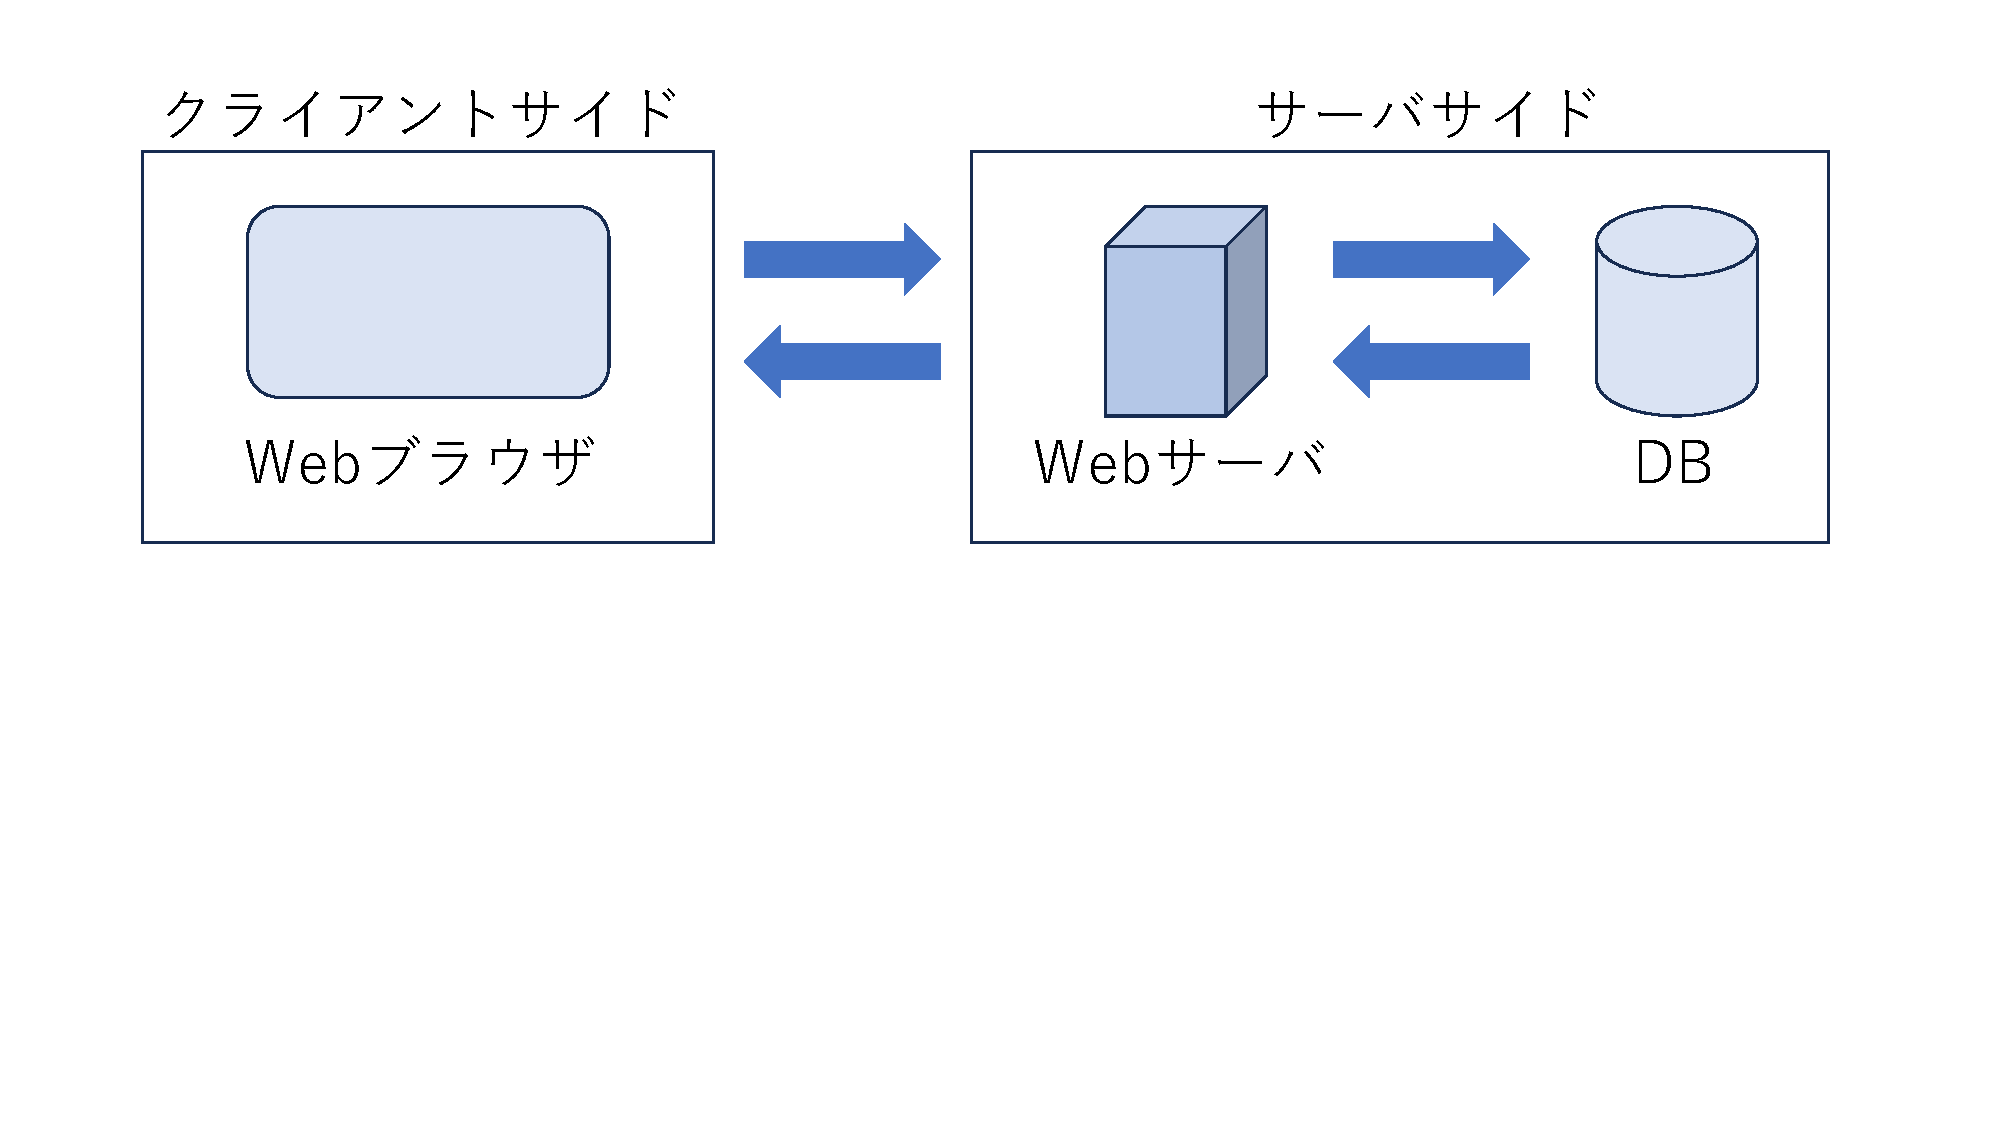
\includegraphics[clip,width=160mm,height=44mm]{images/sa-ba.pdf}
\end{center}
 \caption{開発したシステムの構成}
 \label{fig:sa-ba}
\end{figure}


\subsection{サーバサイド}
\subsubsection{処理内容}
サーバサイドでは,クライアントサイドから送られた情報をもとに,学習者が選択した内容によって表示する評価等を変更する処理を行い,クライアントサイドに結果を返す処理を行う.

\subsubsection{使用している言語}
本学習ツールの開発には,Node.jsのフレームワークの一つであるExpress.jsを利用した.

Node.jsは,サーバーサイドのJavaScript実行環境の一つである.
Node.jsは大量なアクセスに強くリアルタイムの処理に適していること等から,Webアプリケーションの開発等によく使われる.
サーバサイドで学習者の選択によって評価等の表示項目を変更する処理を行うために,サーバーサイドの実行環境であるNode.jsを使用して開発した.

Express.jsはNode.jsのフレームワークの一つである.
Express.jsを利用することで,Node.jsを使用してWebアプリケーションを作成するために必要な機能を容易に実装することができる.
Node.jsを使用した開発を容易にすることを目的として,Express.jsを利用した.

\subsection{DB}
DBには,項目ごとの選択肢や学習者の選択に対する評価に必要な情報等を持たせている.

\subsubsection{DBの設計}
開発したシステムのDBの設計を表\ref{tab:table}に示す.
DBには,textテーブル,colorテーブル,tcテーブル,fontテーブル,evaテーブルの5つのテーブルがある.

\begin{table}[h]
    \caption{テーブル一覧}
   \label{tab:table}
    \centering
    \begin{tabular}{|l||l|l|l|}
        \hline
        テーブル名 & 内容  \\ \hline
        \hline
        text & 項目ごとに表示する文章 \\ \hline
        color & 選択肢となる色の情報 \\ \hline
        tc & 項目と選択肢の対応関係 \\ \hline
        font & 選択肢となるフォントの情報 \\ \hline
        eva & 2色を組み合わせた際の評価 \\ \hline
    \end{tabular}
\end{table}

\subsubsection{DBの詳細}

表\ref{tab:text}はtextテーブルの構成である.
textテーブルには,項目ごとに表示する文章等の情報を格納している.
このテーブルから,評価として表示する文章等を取り出して,学習者に提示している.
idは項目の番号,itemは項目名,queは学習者への指示,goodは学習者の選択が適していた場合の評価,badは適していなかった場合の評価,advはCUDに配慮するためのアドバイスを文章として格納している.

\begin{table}[h]
    \caption{textテーブル}
   \label{tab:text}
    \centering
    \begin{tabular}{|l||l|l|l|}
        \hline
        カラム名 & 内容  \\ \hline
        \hline
        id & 項目番号 \\ \hline
        item & 項目名 \\ \hline
        que & 指示文 \\ \hline
        good & 適した場合の評価 \\ \hline
        bad & 適していない場合の評価 \\ \hline
        adv & アドバイス \\ \hline         
    \end{tabular}
\end{table}

\clearpage
表\ref{tab:color}はcolorテーブルの構成である.
このテーブルには選択肢となる色の情報を格納している.
別色覚での見え方を再現したカラーコード等が入っており,これらのデータを利用して学習者の選択に対して別色覚での見え方を表示している.
idは番号,nameは色の名前,ccodeは色のカラーコード,pcode,dcode,scodeは別色覚での見え方を再現したカラーコードを色覚ごとに格納している.

\begin{table}[h]
    \caption{colorテーブル}
   \label{tab:color}
    \centering
    \begin{tabular}{|l||l|l|l|}
        \hline
        カラム名 & 内容  \\ \hline
        \hline
        id & 番号 \\ \hline
        name & 名前 \\ \hline
        ccode & カラーコード(通常の色覚) \\ \hline
        pcode & カラーコード(P型色覚) \\ \hline
        dcode & カラーコード(D型色覚) \\ \hline
        scode & カラーコード(T型色覚) \\ \hline         
    \end{tabular}
\end{table}

表\ref{tab:tc}はtcテーブルの構成である.
このテーブルは,textテーブルとcolorテーブルの中間テーブルである.
項目ごとに選択肢となる色が異なるため,項目と選択肢の対応関係を格納している.
t-idはtextテーブルのid,c-idはcolorテーブルのidを表す.

\begin{table}[h]
    \caption{tcテーブル}
   \label{tab:tc}
    \centering
    \begin{tabular}{|l||l|l|l|}
        \hline
        カラム名 & 内容  \\ \hline
        \hline
        t-id & 項目番号 \\ \hline
        c-id & 色番号 \\ \hline   
    \end{tabular}
\end{table}

%\clearpage
表\ref{tab:font}はfontテーブルの構成である.
このテーブルには,文字の強調について学ぶ際の選択肢となるフォントの情報を格納している.
idは番号,faceはCSSでフォントを指定する際の値,nameはフォントの名前,gbはCUDに配慮したフォントであるかを0か1で格納している.

\begin{table}[h]
    \caption{fontテーブル}
   \label{tab:font}
    \centering
    \begin{tabular}{|l||l|l|l|}
        \hline
        カラム名 & 内容  \\ \hline
        \hline
        id & 番号 \\ \hline
        face & 値 \\ \hline
        name & 名前 \\ \hline
        gb & 評価 \\ \hline
    \end{tabular}
\end{table}

\clearpage
表\ref{tab:eva}はevaテーブルの構成である.
このテーブルには,2色のカラーコードと組み合わせた際の評価となる情報を格納している.
2色を組み合わせた際に色覚異常の見え方でも区別がつきやすい組み合わせかどうかこのテーブルの情報をもとに判断している.
cola,colbはそれぞれ別のカラーコード,gbはその2色の組み合わせがCUDに配慮されているかを0か1で格納している.

\begin{table}[h]
    \caption{evaテーブル}
   \label{tab:eva}
    \centering
    \begin{tabular}{|l||l|l|l|}
        \hline
        カラム名 & 内容  \\ \hline
        \hline
        cola & カラーコード1 \\ \hline
        colb & カラーコード2 \\ \hline
        gb & 評価 \\ \hline
    \end{tabular}
\end{table}




\subsubsection{使用したDB}
DBにはSQLiteを使用している.
SQLiteはアプリケーションに組み込むことで利用する簡易的なDBである.
主要なデータベースに比べて大規模なWebアプリには不向きな反面,セットアップが容易であるため,本学習ツールではSQLiteを利用した開発を行った.






